% Fig. 6 -- order-unstable rows (argmax identity differs between scored orderings).
% Data: "order_unstable" in
%   bench/results/authored144-...-readout-cyclic-shots3.json      87 / 144  (3 orderings)
%   bench/results/authored144-...-readout-calibrated-shots3.json  80 / 144  (3 orderings)
%   bench/results/authored144-...-readout-full-shots3.json        106 / 144 (6 orderings)
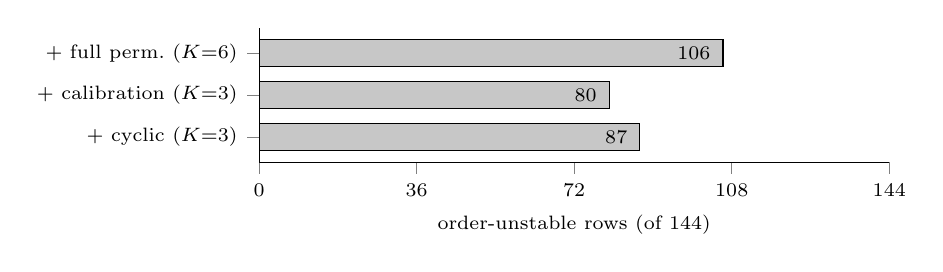
\begin{tikzpicture}
\begin{axis}[
    xbar, scale only axis, width=0.66\columnwidth, height=17mm,
    xmin=0, xmax=144, ymin=0.4, ymax=3.6, y dir=reverse, bar width=3.4mm,
    ytick={1,2,3},
    yticklabels={{+ full perm.\ ($K{=}6$)},{+ calibration ($K{=}3$)},{+ cyclic ($K{=}3$)}},
    yticklabel style={font=\scriptsize}, xticklabel style={font=\scriptsize},
    xtick={0,36,72,108,144},
    xlabel={order-unstable rows (of 144)}, xlabel style={font=\scriptsize},
    nodes near coords, every node near coord/.append style={font=\scriptsize, anchor=east, xshift=-1pt},
    axis lines*=left, tick align=outside]
  \addplot[draw=black, fill=black!22] coordinates {(106,1) (80,2) (87,3)};
\end{axis}
\end{tikzpicture}
